\documentclass[a4paper,12pt]{report}

\usepackage{cmap}
\usepackage[T2A]{fontenc}
\usepackage[utf8]{inputenc}
\usepackage[english,russian]{babel}
\usepackage{listings}
\usepackage{amsmath}
\usepackage{float}
\usepackage{csquotes}
\usepackage{mathtools}
\usepackage{hyphenat}
\usepackage{amsfonts}
\usepackage{upgreek}

\usepackage{xcolor}
\usepackage{hyperref}

\usepackage{graphicx}
\graphicspath{ {./images/} }

\definecolor{dkgreen}{rgb}{0,0.6,0}
\definecolor{gray}{rgb}{0.5,0.5,0.5}
\definecolor{mauve}{rgb}{0.58,0,0.82}

\lstset{
    language=Python,               
    basicstyle=\small\sffamily, 
    numbers=left,           
    numberstyle=\tiny,        
    stepnumber=1,               
    numbersep=5pt,                  
    aboveskip=3mm,
    belowskip=3mm,
    showstringspaces=false,
    columns=flexible,
    captionpos=b, 
    basicstyle={\small\ttfamily},
    numbers=left,
    numberstyle=\tiny\color{gray},
    keywordstyle=\color{blue},
    commentstyle=\color{mauve},
    stringstyle=\color{dkgreen},
    breaklines=true,
    breakatwhitespace=true,
    tabsize=3
}

\title{Лабораторная работа №6\\Дискретное косинусное преобразование}
\author{Крынский Павел}
\date{\today}

\begin{document}

\maketitle
\tableofcontents
\listoffigures
\lstlistoflistings

\maketitle

\chapter{Упражнение 6.1}

Я добавил тестирующую функцию и функцию для оценки наклона графиков:

\begin{lstlisting}[caption=Тестирующая функция и функция для оценки наклона графиков]
def speed_test(ns, func):
    res = []
    for N in ns:
        print(N)
        ts = (0.5 + np.arange(N)) / N
        freqs = (0.5 + np.arange(N)) / 2
        ys = noise.ys[:N]
        result = %timeit -r1 -o func(ys, freqs, ts)
        res.append(result)
        
    bests = [result.best for result in res]
    return bests

def fit_slope(ns, bests): 
    x = np.log(ns)
    y = np.log(bests)
    t = linregress(x,y)
    slope = t[0]

    return slope
\end{lstlisting}

    Далее я создал сигнал, на котором будет происходить тестирование и массив со степенями двойки с 4-ой по 11-ю.
    

\begin{lstlisting}[caption=Массив степеней двойки]
signal = thinkdsp.UncorrelatedGaussianNoise()
noise = signal.make_wave(duration=1.0, framerate=16384)
ns = 2** np.arange(4,12)
\end{lstlisting}

Ниже я привел резульиаты запуска тестирующей функции для трех функций(analyze1, analyze2, fftpack.dct):   

\begin{lstlisting}[caption=Результат работы, literate={µ}{$\upmu$}1 {±}{$\pm$}2]
16
24.9 µs ± 0 ns per loop (mean ± std. dev. of 1 run, 10000 loops each)
32
44.8 µs ± 0 ns per loop (mean ± std. dev. of 1 run, 10000 loops each)
64
106 µs ± 0 ns per loop (mean ± std. dev. of 1 run, 10000 loops each)
128
352 µs ± 0 ns per loop (mean ± std. dev. of 1 run, 1000 loops each)
256
1.68 ms ± 0 ns per loop (mean ± std. dev. of 1 run, 1000 loops each)
512
9.8 ms ± 0 ns per loop (mean ± std. dev. of 1 run, 100 loops each)
1024
40.5 ms ± 0 ns per loop (mean ± std. dev. of 1 run, 10 loops each)
2048
191 ms ± 0 ns per loop (mean ± std. dev. of 1 run, 10 loops each)

16
14.9 µs ± 0 ns per loop (mean ± std. dev. of 1 run, 100000 loops each)
32
24.6 µs ± 0 ns per loop (mean ± std. dev. of 1 run, 10000 loops each)
64
57 µs ± 0 ns per loop (mean ± std. dev. of 1 run, 10000 loops each)
128
177 µs ± 0 ns per loop (mean ± std. dev. of 1 run, 10000 loops each)
256
660 µs ± 0 ns per loop (mean ± std. dev. of 1 run, 1000 loops each)
512
4.16 ms ± 0 ns per loop (mean ± std. dev. of 1 run, 100 loops each)
1024
17 ms ± 0 ns per loop (mean ± std. dev. of 1 run, 100 loops each)
2048
63.8 ms ± 0 ns per loop (mean ± std. dev. of 1 run, 10 loops each)

16
8.18 µs ± 0 ns per loop (mean ± std. dev. of 1 run, 100000 loops each)
32
7.91 µs ± 0 ns per loop (mean ± std. dev. of 1 run, 100000 loops each)
64
8.11 µs ± 0 ns per loop (mean ± std. dev. of 1 run, 100000 loops each)
128
9.56 µs ± 0 ns per loop (mean ± std. dev. of 1 run, 100000 loops each)
256
8.77 µs ± 0 ns per loop (mean ± std. dev. of 1 run, 100000 loops each)
512
10.3 µs ± 0 ns per loop (mean ± std. dev. of 1 run, 100000 loops each)
1024
12.5 µs ± 0 ns per loop (mean ± std. dev. of 1 run, 100000 loops each)
2048
17.7 µs ± 0 ns per loop (mean ± std. dev. of 1 run, 100000 loops each)
\end{lstlisting}

Также приведу показатели уклона трех функций:
1.9205374674429947
1.8105335861011087
0.14312061938412077

И для наглядности я вывыел три графика для сравнения:

\begin{figure}[H]
        \centering
        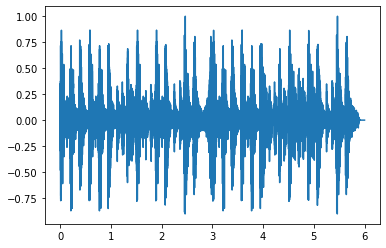
\includegraphics[width=0.75\textwidth]{1.png}
        \caption{Визуализация данных}
        \label{fig:lab6_fig1_1}
\end{figure}

У функции fftpack.dct лучшие временные траты. 

\chapter{Упражнение 6.2}

Берем нашу запис сегмент, а затем ДКП этого сегмента:

\begin{lstlisting}[caption=Загрузка звука и сегмент]
wave = thinkdsp.read_wave('185347__lemoncreme__symphony-sounds.wav')
wave.make_audio()
sg = wave.segment(start=1.2, duration=0.5)
sg.normalize()
sg.make_audio()
sg_dct = sg.make_dct()
sg_dct.plot(high=1000)
decorate(xlabel='Frequency (Hz)', ylabel='DCT')
\end{lstlisting}

\begin{figure}[H]
        \centering
        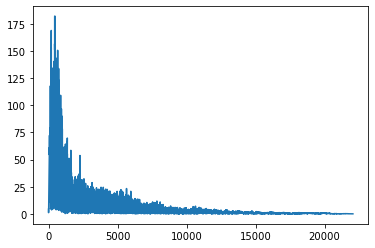
\includegraphics[width=0.75\textwidth]{2.png}
        \caption{Визуализация сжатого звука}
        \label{fig:lab6_fig2_1}
\end{figure}

Многие записи близки к нулю. Следующая функция принимает ДКП и устанавливает для элементов ниже порога значение 0.

\begin{lstlisting}[caption=Функция \texttt{compress}]
def compress(dct, thresh=1):
    count = 0
    for i, amp in enumerate(dct.amps):
        if np.abs(amp) < thresh:
            dct.hs[i] = 0
            count += 1
            
    n = len(dct.amps)
    print(count, n, 100 * count / n, sep='\t')
\end{lstlisting}

Если мы применим его к сегменту, мы можем удалить более 90\% элементов:

\begin{lstlisting}[caption=Сжатие звука]
sg_dct = sg.make_dct()
compress(sg_dct, thresh=10)
sg_dct.plot(high=1000)
\end{lstlisting}

\begin{figure}[H]
        \centering
        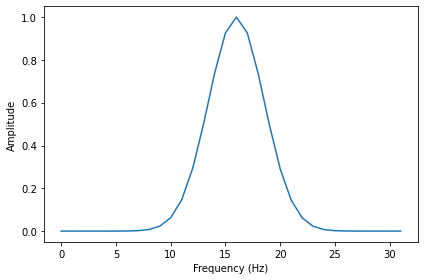
\includegraphics[width=0.75\textwidth]{3.png}
        \caption{Визуализация сжатого звука}
        \label{fig:lab6_fig2_2}
\end{figure}

\begin{lstlisting}[caption=Воспроизведение сжатого звука]
sg2 = sg_dct.make_wave()
sg2.make_audio()
\end{lstlisting}

Результат звучит точно так же.

Чтобы сжать более длинный сегмент, мы можем сделать спектрограмму ДКП. 

\begin{lstlisting}[caption=Функция \texttt{make\_dct\_spectrogram}]
def make_dct_spectrogram(wave, seg_length):
    window = np.hamming(seg_length)
    i, j = 0, seg_length
    step = seg_length

    spec_map = {}

    while j < len(wave.ys):
        segment = wave.slice(i, j)
        segment.window(window)

        t = (segment.start + segment.end) / 2
        spec_map[t] = segment.make_dct()

        i += step
        j += step

    return thinkdsp.Spectrogram(spec_map, seg_length)
\end{lstlisting}

Теперь мы можем составить DCT-спектрограмму и применить сжатие к каждому сегменту:

\begin{lstlisting}[caption=Сжатие звука]
spectro = make_dct_spectrogram(wave, seg_length=1024)
for t, dct in sorted(spectro.spec_map.items()):
    compress(dct, thresh=0.2)
\end{lstlisting}

В большинстве сегментов сжатие составляет 75-80\%. Чтобы услышать, как это звучит, мы можем преобразовать спектрограмму обратно в волну и воспроизвести её.

\begin{lstlisting}[caption=Воспроизведение сжатого звука]
wave2 = spectro.make_wave()
wave2.make_audio()
\end{lstlisting}

Так же прослушаем оригинал для сравнения.

\begin{lstlisting}[caption=Воспроизведение оригинального звука]
wave.make_audio()
\end{lstlisting}

При сжатии слышно характерный треск во время воспроизведения аудио, так что можно смело сказать, что нам удалось сжать аудиозапись.

\chapter{Упражнение 6.3}

 Теперь нам нужно запустить готовый \sloppy{\texttt{phase.ipynb}} и посмотреть, что там происходит.
    
    Если мы посмотрим на фазовые сдвиги каждой компоненты некоторого звука, то мы будем видеть только много случайных значений, однако если отфильтровать частоты с маленьким амплитудами, то начнет вырисовываться струкутра. Величина фазы от частоты компоненты может зависеть как линейно, так и случайно, однако в подавляющем большинстве случаев ухо не будет способно это воспринять.
    
    

\chapter{Выводы}

Во время выполнения лабораторной работы получены навыки работы с прямым и обратным дискретным косинусным преобразованием. Также получены навыки их практического применения.

\end{document}